\documentclass[conference]{IEEEtran}

\usepackage[T1]{fontenc}
\usepackage[utf8]{inputenc}
\usepackage{microtype}
\usepackage{graphicx}
\usepackage{booktabs}
\usepackage{amsmath,amssymb,amsfonts}
\usepackage{hyperref}
\usepackage{xcolor}
\usepackage{listings}
\usepackage{cite}
\usepackage{tikz}
\usetikzlibrary{arrows.meta,positioning}

\hypersetup{
  colorlinks=true,
  linkcolor=blue,
  urlcolor=blue,
  pdftitle={Home Assignment 1: Image Processing for Handwritten Digit Recognition}
}

\lstset{
  basicstyle=\ttfamily\small,
  breaklines=true,
  frame=single,
  columns=fullflexible
}

\title{Home Assignment 1: Image Processing for Handwritten Digit Recognition}
\author{\IEEEauthorblockN{Jordán Fernández Ruiz}
\IEEEauthorblockA{UNI-ID: \texttt{262754IV}\\
Tallinn University of Technology}}

\begin{document}
\setlength{\parindent}{0pt}
\setlength{\parskip}{0.35em}
\maketitle

\begin{abstract}
This report presents an image-processing pipeline for handwritten digit recognition. The main contribution is the deterministic preprocessing stage that converts a digit image into the representation required by the classifier. It includes normalization, spatial resizing, block averaging, downsampling, and integer representation. The intermediate images generated by the project make the effect of each operation visible. A compact CNN is then used as the learned feature extractor for the final $28 \times 28$ grayscale representation.
\end{abstract}

\begin{IEEEkeywords}
image processing, preprocessing, spatial filtering, downsampling, handwritten digit recognition
\end{IEEEkeywords}

\section{Introduction}
The selected application domain is image processing, specifically handwritten number recognition. This domain is suitable because digit images are small, the signal-processing pipeline is well defined, and the transformations can be inspected visually at every stage.

The selected application is handwritten number recognition. The practical goal is to transform a digit image into a representation suitable for classification while preserving its important strokes and shapes. The project also demonstrates that feature extraction can be performed by convolutional layers, in addition to deterministic image-processing operations.

The C/C++ implementation is an optional embedded deployment of the image-processing pipeline. The main assignment evaluation focuses on preprocessing and intermediate image comparisons.

\section{System Overview}
Figure~\ref{fig:pipeline} describes the implemented pipeline.

\begin{figure}[ht]
\centering
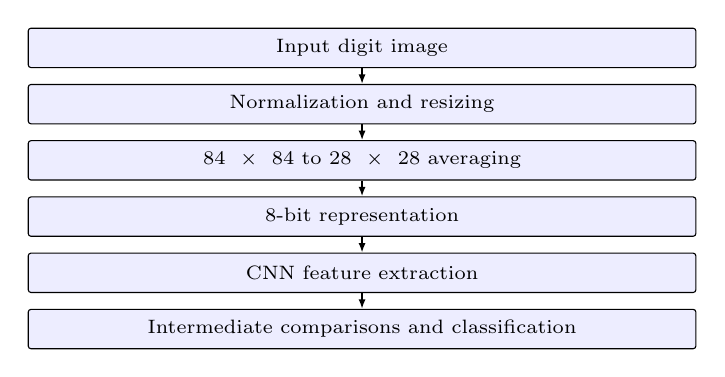
\begin{tikzpicture}[
  node distance=2mm,
  stage/.style={draw, rounded corners=1pt, align=center, minimum height=5mm,
    text width=0.68\columnwidth, font=\scriptsize, fill=blue!7},
  arrow/.style={-{Latex[length=1.2mm]}, semithick}
]
\node[stage] (touch) {Input digit image};
\node[stage, below=of touch] (buffer) {Normalization and resizing};
\node[stage, below=of buffer] (image) {$84 \times 84$ to $28 \times 28$ averaging};
\node[stage, below=of image] (quant) {8-bit representation};
\node[stage, below=of quant] (cnn) {CNN feature extraction};
\node[stage, below=of cnn] (result) {Intermediate comparisons and classification};
\draw[arrow] (touch) -- (buffer);
\draw[arrow] (buffer) -- (image);
\draw[arrow] (image) -- (quant);
\draw[arrow] (quant) -- (cnn);
\draw[arrow] (cnn) -- (result);
\end{tikzpicture}
\caption{Image preprocessing pipeline and optional classification stage.}
\label{fig:pipeline}
\end{figure}

The image-processing evaluation is independent of the final hardware demonstration. The comparison figures are generated from the scikit-learn handwritten-digit samples and show the intermediate outputs of the preprocessing pipeline. The classifier is treated as the final stage; the focus of this assignment is how the input image is transformed before classification.

\section{Image Processing and Feature Extraction}
\subsection{Preprocessing pipeline}
The preprocessing pipeline has four main purposes: preserve the digit structure, reduce the amount of data, remove small isolated variations, and match the input format expected by the CNN. The complete sequence is:

\begin{enumerate}
\item Normalize the source intensities to the range $[0,1]$.
\item Resize the source image to the classifier resolution of $28 \times 28$ pixels.
\item Average each local $3 \times 3$ region when converting the larger touch buffer to the classifier resolution.
\item Quantize the normalized image to the model's \texttt{int8} representation.
\end{enumerate}

The first two operations are used for the training samples, while the block averaging operation describes the runtime touchscreen path. Both paths produce the same final spatial resolution, allowing the CNN to process a fixed-size input.

\subsection{Touch image acquisition}
The touchscreen stores the handwritten stroke in an $84 \times 84$ binary buffer. A black stroke is represented by active pixels and the background remains zero. A single drawing region was chosen because it makes the interaction more simple and avoided unreliable button presses on the touchscreen.

\subsection{Spatial reduction}
The CNN expects an image of $28 \times 28$ pixels. Therefore, the $84 \times 84$ drawing is reduced by a factor of three in both directions. For every output pixel, the implementation averages a local $3 \times 3$ region:

\[
I_{28}(i,j) = \frac{1}{9}\sum_{u=0}^{2}\sum_{v=0}^{2} I_{84}(3i+u,3j+v).
\]

The value is then scaled to the integer range $[0,255]$. This operation is a useful signal-processing step because it reduces the input size, smooths sparse touch points, and makes the drawn signal compatible with the training resolution.

\subsection{Intermediate output comparison}
Figure~\ref{fig:preprocessing-comparison} compares the main intermediate representations for one digit. The original $8 \times 8$ sample is normalized and resized to $28 \times 28$. An $84 \times 84$ touch-like representation is then reduced using the same $3 \times 3$ averaging idea used by the touchscreen path. The final panel shows the effect of representing the image with 8-bit values. This comparison makes the spatial filtering and information-preserving parts of the pipeline visible rather than treating preprocessing as a hidden step.

\begin{figure}[ht]
\centering
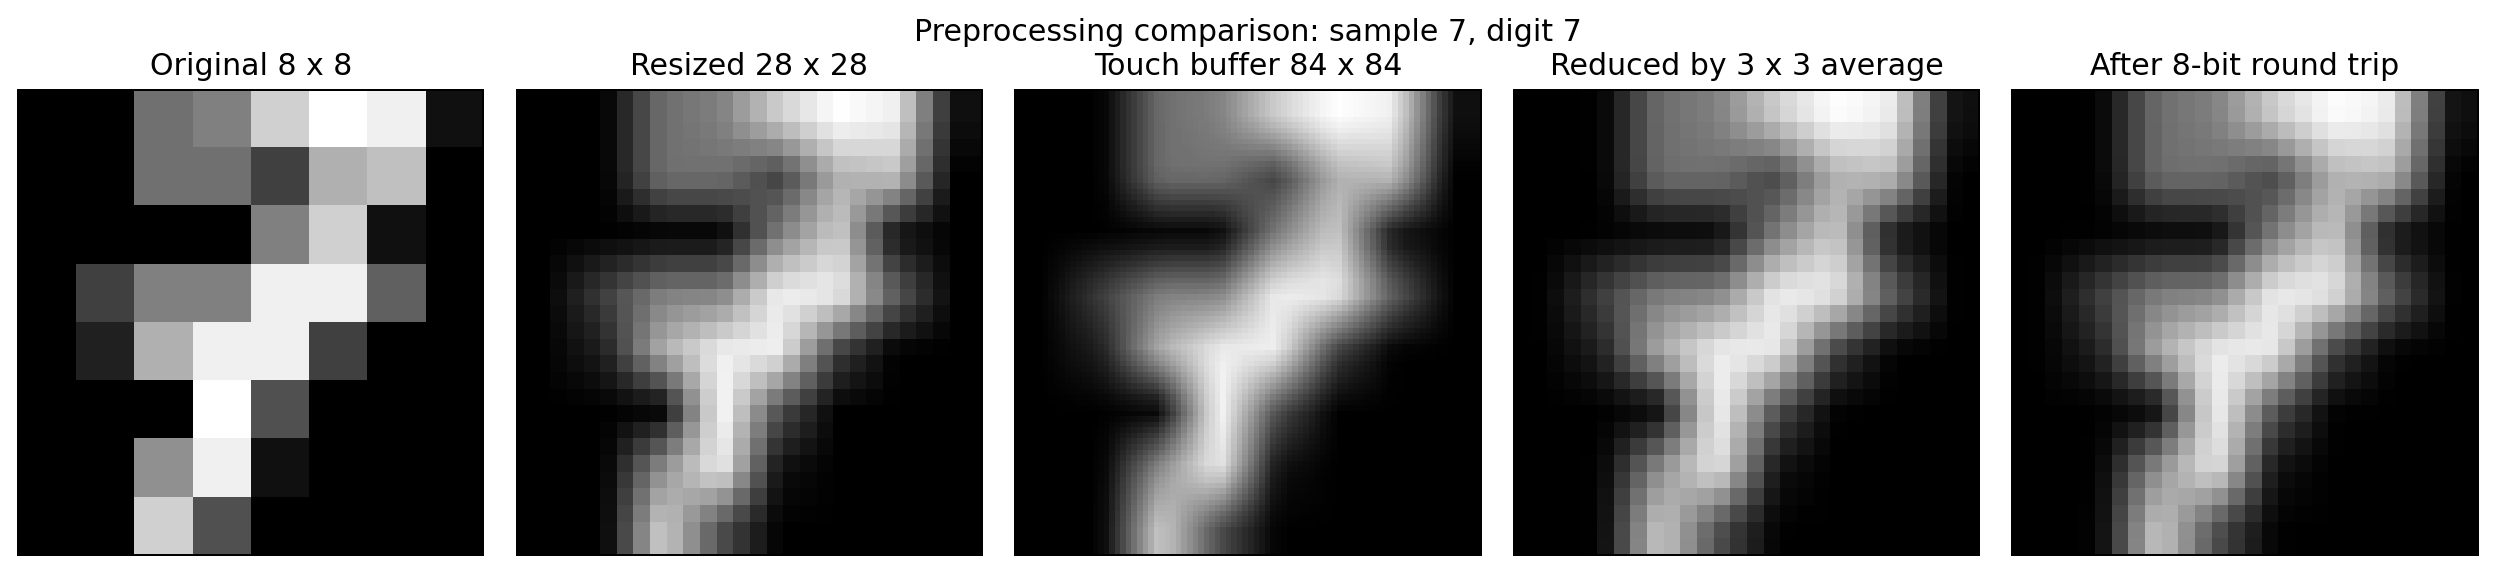
\includegraphics[width=\columnwidth]{images/preprocessing/digit_7_pipeline.png}
\caption{Intermediate outputs of the image preprocessing pipeline for digit 7.}
\label{fig:preprocessing-comparison}
\end{figure}

\subsection{Filter comparison and signal metrics}
To evaluate the spatial filter quantitatively, the filtered image is resized back to $84 \times 84$ and compared with the original touch-like signal. The experiment uses mean squared error (MSE), root mean squared error (RMSE), mean absolute error (MAE), peak signal-to-noise ratio (PSNR), signal correlation, and gradient RMSE. Gradient RMSE measures changes in local edges and therefore complements pixel-wise error metrics.

\begin{equation*}
\mathrm{MSE}=\frac{1}{N}\sum_{i=1}^{N}(x_i-y_i)^2,
\qquad
\mathrm{PSNR}=10\log_{10}\left(\frac{1}{\mathrm{MSE}}\right).
\end{equation*}

Table~\ref{tab:filter-results} compares three average-filter sizes. The $3 \times 3$ filter is the selected operation because it smooths the signal while preserving substantially more structure than the larger $5 \times 5$ filter.

\begin{table}[ht]
\centering
\caption{Spatial filtering comparison for digit 7.}
\label{tab:filter-results}
\begin{tabular}{lccccc}
\toprule
Filter & MSE & MAE & PSNR (dB) & Corr. & Grad. RMSE \\
\midrule
$2 \times 2$ & 0.000035 & 0.002862 & 44.54 & 0.9998 & 0.002820 \\
$3 \times 3$ & 0.000065 & 0.004856 & 41.89 & 0.9998 & 0.002336 \\
$5 \times 5$ & 0.009091 & 0.065237 & 20.41 & 0.9516 & 0.013683 \\
\bottomrule
\end{tabular}
\end{table}

\begin{figure}[ht]
\centering
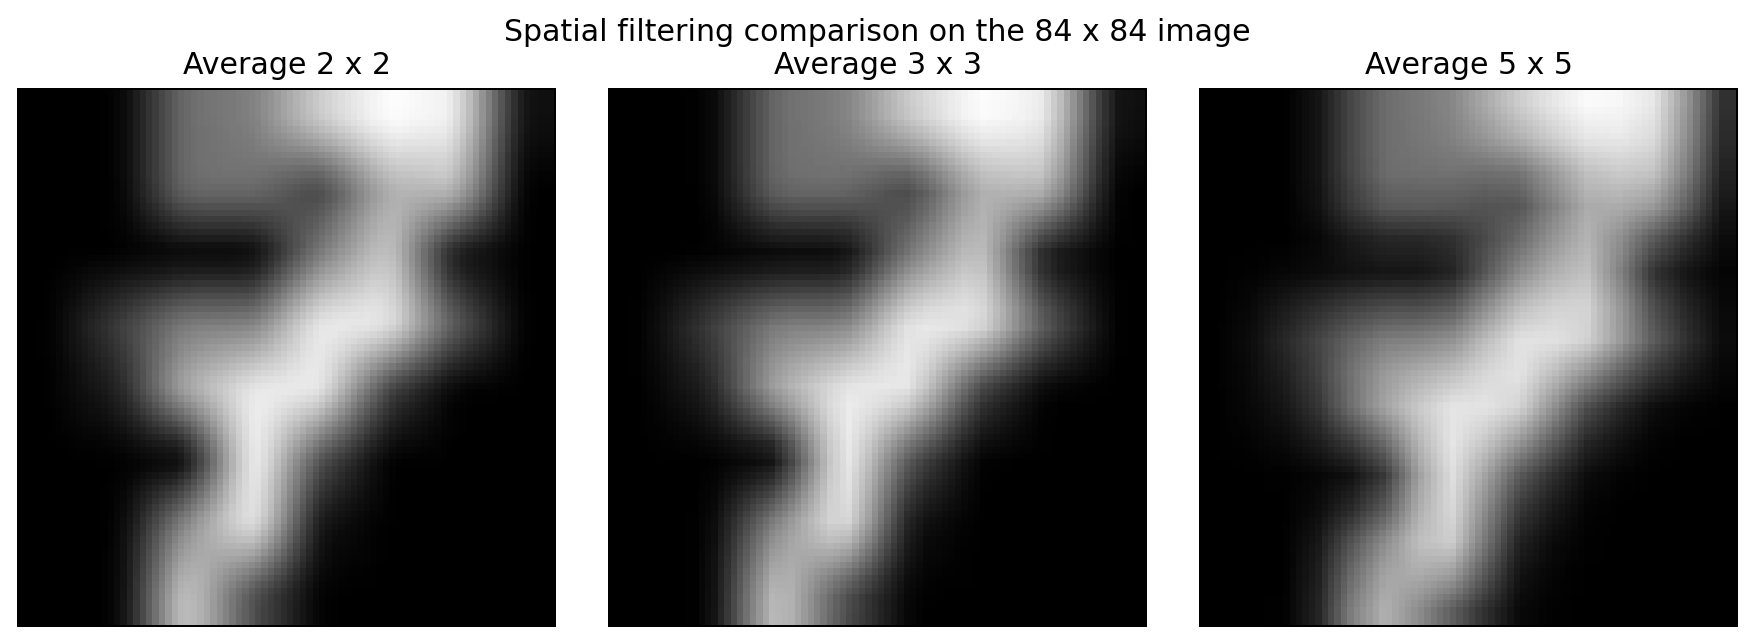
\includegraphics[width=\columnwidth]{images/preprocessing/filter_comparison.png}
\caption{Comparison of average-filter sizes applied to the $84 \times 84$ signal.}
\label{fig:filter-comparison}
\end{figure}

\subsection{Normalization and quantization}
Before inference, each pixel is normalized as

\[
x_{norm} = \frac{x}{255}.
\]

The input tensor is fully quantized. The normalized value is mapped to the tensor representation by

\[
x_q = \operatorname{clip}\left(\operatorname{round}\left(\frac{x_{norm}}{s}\right) + z, -128, 127\right),
\]

where $s$ is the input scale and $z$ is the input zero point read from the TFLite model. Reading these parameters from the model avoids using hard-coded quantization constants. This stage is important because the embedded model expects \texttt{int8} data, while the touchscreen initially provides unsigned pixel values.

\subsection{Effect of the preprocessing operations}
The deterministic operations have complementary effects. Resizing changes the spatial resolution while interpolating between neighboring pixels. The $3 \times 3$ average acts as a low-pass spatial filter: it suppresses isolated touch points and preserves broader stroke structure. Normalization removes dependence on the original intensity scale. Finally, \texttt{int8} representation reduces the numerical precision and memory required by the embedded model.

These preprocessing stages are intentionally simple. More classical alternatives such as Sobel edges, histogram of oriented gradients, connected components, or image moments were not used, because the compact CNN can learn stroke, edge, and shape features directly from the normalized image. Therefore, the final system combines downsampling, smoothing, normalization, and quantization with learned feature extraction in the convolutional layers. This was a reasonable trade-off for the available Flash memory and processing resources.

\subsection{CNN feature extraction}
The CNN architecture is shown in Table~\ref{tab:architecture}. The two convolutional layers learn local structures such as stroke direction, corners, curves, and combinations of strokes. Max-pooling reduces the spatial resolution while preserving stronger activations. In this project, convolution and max pooling are the main feature-extraction algorithms.

\begin{table}[ht]
\centering
\caption{Compact CNN used for digit recognition.}
\label{tab:architecture}
\begin{tabular}{ll}
\toprule
Stage & Configuration \\
\midrule
Input & $28 \times 28 \times 1$ grayscale image \\
Convolution 1 & 8 filters, $3 \times 3$, ReLU \\
Max pooling 1 & default Keras pooling configuration \\
Convolution 2 & 16 filters, $3 \times 3$, ReLU \\
Max pooling 2 & default Keras pooling configuration \\
Reshape & $5 \times 5 \times 16 = 400$ features \\
Dense layer & 32 neurons, ReLU \\
Output layer & 10 neurons, softmax \\
\bottomrule
\end{tabular}
\end{table}

The final softmax layer produces one score for each digit class from 0 to 9. The predicted digit is the class with the highest score. The displayed confidence is the dequantized score of this winning class. It should not be confused with the total classification accuracy of the system.

\section{Optional CNN Extension}
The development dataset was the scikit-learn handwritten digits dataset, obtained through the \texttt{sklearn.datasets.load\_digits()} function. Original $8 \times 8$ images were normalized and resized to $28 \times 28$ so that they matched the touchscreen input format. The data was split with stratification, using 20\% as the validation set.

No pre-trained model or downloaded weights were used. The CNN architecture was created locally in TensorFlow with randomly initialized weights, then trained from scratch for 20 epochs using the Adam optimizer and sparse categorical cross entropy. The complete training and conversion procedure is available in \texttt{tools/train\_quantized\_model.py}. Therefore, the embedded weights in the final \texttt{.tflite} file were produced by this project from the scikit-learn digit samples.

After training, the model was converted to a fully integer TensorFlow Lite model. A representative subset of 200 training images was used by the converter. The input and output tensor types were set to \texttt{int8}. The resulting model uses only the following operations:

\begin{lstlisting}
CONV_2D, MAX_POOL_2D, RESHAPE, FULLY_CONNECTED, SOFTMAX
\end{lstlisting}

These operations were registered explicitly in the TensorFlow Lite Micro resolver. The generated model was embedded as a C byte array in the firmware, aligned to eight bytes.

\section{Optional Model Comparison}
Three CNN configurations were trained with the same stratified 80/20 split, 20 epochs, batch size 64, Adam optimizer, and fully \texttt{int8} conversion. The number of convolution filters and dense neurons were varied to evaluate the accuracy--memory trade-off. Table~\ref{tab:experiments} shows the measured validation accuracy and exported TFLite size.

\begin{table}[ht]
\centering
\caption{CNN parameter experiment results.}
\label{tab:experiments}
\begin{tabular}{lccc}
\toprule
Model & Filters & Validation accuracy & Size \\
\midrule
Small & 4, 8 & 92.78\% & 9,640 B \\
Selected & 8, 16 & 96.11\% & 21,080 B \\
Large & 12, 24 & 96.67\% & 39,504 B \\
\bottomrule
\end{tabular}
\end{table}

The small model is compact, but its accuracy reduction is visible. The large model improves validation accuracy by only 0.56 percentage points over the selected configuration while requiring about 18 kB more Flash memory. The selected configuration was therefore chosen as the better balance for the Pico. The deployed model was generated in a separate final run of this selected configuration; it occupies 20,152 bytes and reached 96.39\% validation accuracy. It has one $1 \times 28 \times 28 \times 1$ \texttt{int8} input tensor and one $1 \times 10$ \texttt{int8} output tensor.

The final model file was measured at 20,152 bytes (19.68 KiB). For comparison, the small and large experimental models occupied 9,640 bytes and 39,504 bytes respectively. These model measurements provide context for the optional embedded deployment; the main comparison in this assignment is the visual change between preprocessing stages.

\section{Discussion}
The implementation meets the assignment requirement because it applies signal-processing algorithms from the image-processing domain. Resizing and normalization create a consistent representation, while average filtering and downsampling reduce the spatial signal. The MSE, RMSE, PSNR, and generated figures provide direct qualitative and quantitative evidence of the intermediate outputs. The CNN and embedded firmware are optional extensions that demonstrate how the processed signal can be used for digit classification.

One limitation is that the model was trained on digit samples resized from $8 \times 8$ images, while a practical input may originate from a larger freehand drawing. The intermediate comparison highlights this domain difference and shows why downsampling and normalization are necessary. More samples collected from the same input source, as well as centering and stroke-thickness normalization, would probably improve robustness.

\section{Conclusion}
A complete image-processing pipeline was implemented and evaluated through intermediate image comparisons. It combines normalization, bilinear resizing, spatial averaging, downsampling, and 8-bit representation. Comparing average filters shows that the $3 \times 3$ operation provides a practical balance between smoothing and preservation of signal structure. The CNN and Pico firmware remain optional extensions for classifying the processed images.

\begin{thebibliography}{00}
\bibitem{tensorflow} TensorFlow, ``TensorFlow Lite for Microcontrollers,'' \url{https://www.tensorflow.org/lite/microcontrollers}.
\bibitem{sklearn} F. Pedregosa et al., ``Scikit-learn: Machine Learning in Python,'' \emph{Journal of Machine Learning Research}, vol. 12, pp. 2825--2830, 2011.
\bibitem{pico} Raspberry Pi Ltd., ``Raspberry Pi Pico Datasheet,'' 2021.
\end{thebibliography}

\end{document}
